\documentclass{article}
\usepackage{hyperref}
\usepackage{graphicx}
\begin{document}
\title{WebPlotDigitizer User Manual\\ Version 2.6}
\author{Ankit Rohatgi\footnote{E-Mail: ankitrohatgi@hotmail.com}}
\maketitle
\tableofcontents

\section{Introduction}
WebPlotDigitizer is a web based software to be used for extracting numeric values from plots and figures.

\begin{figure}
\centering
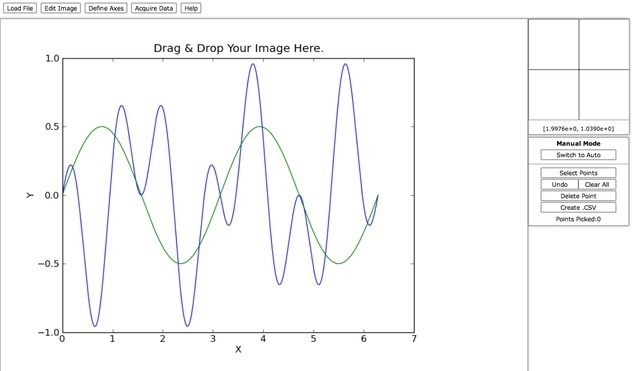
\includegraphics[width=4in]{./figures/testSmall.jpg}
\end{figure}
\subsection{User Manual}
\subsection{Other Resources}
\subsection{License}
WebPlotDigitizer is distributed under GNU General Public License version 3.
\subsection{Source Code}
\subsection{Availability}
Go to the website, \url{http://arohatgi.info/WebPlotDigitizer}.
\subsection{Supported Browsers}
Google Chrome, Mozilla Firefox, Internet Explorer 10, Safari 6.0

\section{Loading Plots}
File, Load
\section{Axes Types}
\subsection{XY Plots}
\subsection{Maps}
\subsection{Image}
\subsection{Polar Plots}
\subsection{Ternary Phase Diagrams}
\subsection{Data Acquisition}
\section{Data Acquisition}
\subsection{Manual Mode}
\subsection{Automatic Mode}
\subsubsection{Foreground Color (FG)}
\subsubsection{Background Color (BG)}
\subsubsection{Mark Region}
\subsection{Digitization Algorithms}
\section{CSV Data}
\end{document}
